% !TEX root = main.tex

\section{Yields determination}
\label{sec:massFits}

An extended unbinned maximum likelihood fit to the reconstructed $B_s$ mass of the selected events is performed in order to determine the signal and background yields.
The invariant mass $m(D_s h \pi \pi)$ is determined from a DTF constraining the mass of the $D_s$ to the PDG value and the position of the PV. 
The probability density functions (PDFs) used to describe the signal and background components are described in the following.

Due to different mass resolutions, we perform the invariant mass fits simultaneously for each data-taking period and each trigger category. 
We further introduce four $D_s$ final state categories:
$D_s \to \phi \pi$, $D_s \to K^*(892) \pi$, $D_s \to \pi \pi \pi$ and $D_s \to K h \pi$
to account for different signal purities. 
The $D_s \to K h \pi$ category combines the two $D_s$ decay channels with the lowest statistics: $D_s \to K K \pi$ (non-resonant) and $D_s \to K \pi \pi$.
This amounts to 16 categories in total.
%After the full selection we assume that the resulting sample is composed of the following
%components:
%226 ? the signal (D0 ? K?K+?+??, D0 ? ?????+?? or D0 ? K??+?+?? decays);
%227 ? peaking background from 4-body hadronic D0 ? h+h(?)??+?? decays, where the
%228 two pions are both misidentified as muons;
%229 ? combinatorial background.


\subsection{Signal model}
\label{subsec:signalModel}

The signal $B_s$-mass distribution of both $\Bs\to\Ds\kaon\pion\pion$ and $\Bs\to\Ds\pion\pion\pion$  is modeled using a Johnson's SU function \cite{10.2307/2332539}, which 
results from a variable transformation of a normal distribution to allow for asymmetric tails:
\begin{align}
\mathcal J(x\vert\mu,\sigma,\nu,\tau) &=
\frac{e^{- \frac{1}{2} r^2}}{2\pi \cdot c \cdot \sigma \cdot \tau \cdot \sqrt{z^2+1}} \\
% \frac{\delta}{\sigma 2\pi \sqrt{1+(\frac{m_{\Bs}-\mu}{\sigma})^{2}}} exp \left(-\frac{1}{2}[\gamma + \delta Argsh (\frac{m_{\Bs} - \mu}{\sigma})^{2}]\right).
r &= - \nu + \frac{\text{asinh}(z)}{\tau} \\
z & = \frac{x-(\mu - c \cdot \sigma \cdot e^\tau \text{sinh}(\nu\cdot \tau)}{c \cdot \tau} \\
c &= \frac{e^{\tau^2}-1}{2\sqrt{e^{\tau^2} \cdot \text{cosh}(2 c \cdot \tau)+1}} .
\label{eq:RooJohnsonSU}
\end{align}
It is conveniently expressed in terms of the central moments up to order four: 
The mean of the distribution $\mu$, the standard deviation $\sigma$,
the skewness $\nu$ and the kurtosis $\tau$.
%The sign of $\gamma$ in Eq. \ref{eq:RooJohnsonSU} determines whether the tail is located at lower ($\gamma > 0$) or higher ($\gamma < 0$) invariant mass values than the mean $\mu$ of the gaussian function 
%and $\delta$ describes the (a)symmetry of the fitted distribution. Higher values of $\delta$ result in a more symmetric, gaussian-like function.  
%Another Johnson SU function function is used to account for the contribution of the $\B^{0}\to\Ds\kaon\pion\pion$ decay, which is also present in the $m(\Ds\kaon\pion\pion)$ spectrum.
The tail parameters $\nu$ and $\tau$ are fixed to the values obtained by a fit to the invariant mass distribution of simulated events shown in Fig~\ref{fig: BsMassShapes}. 
\begin{figure}[h]
\centering
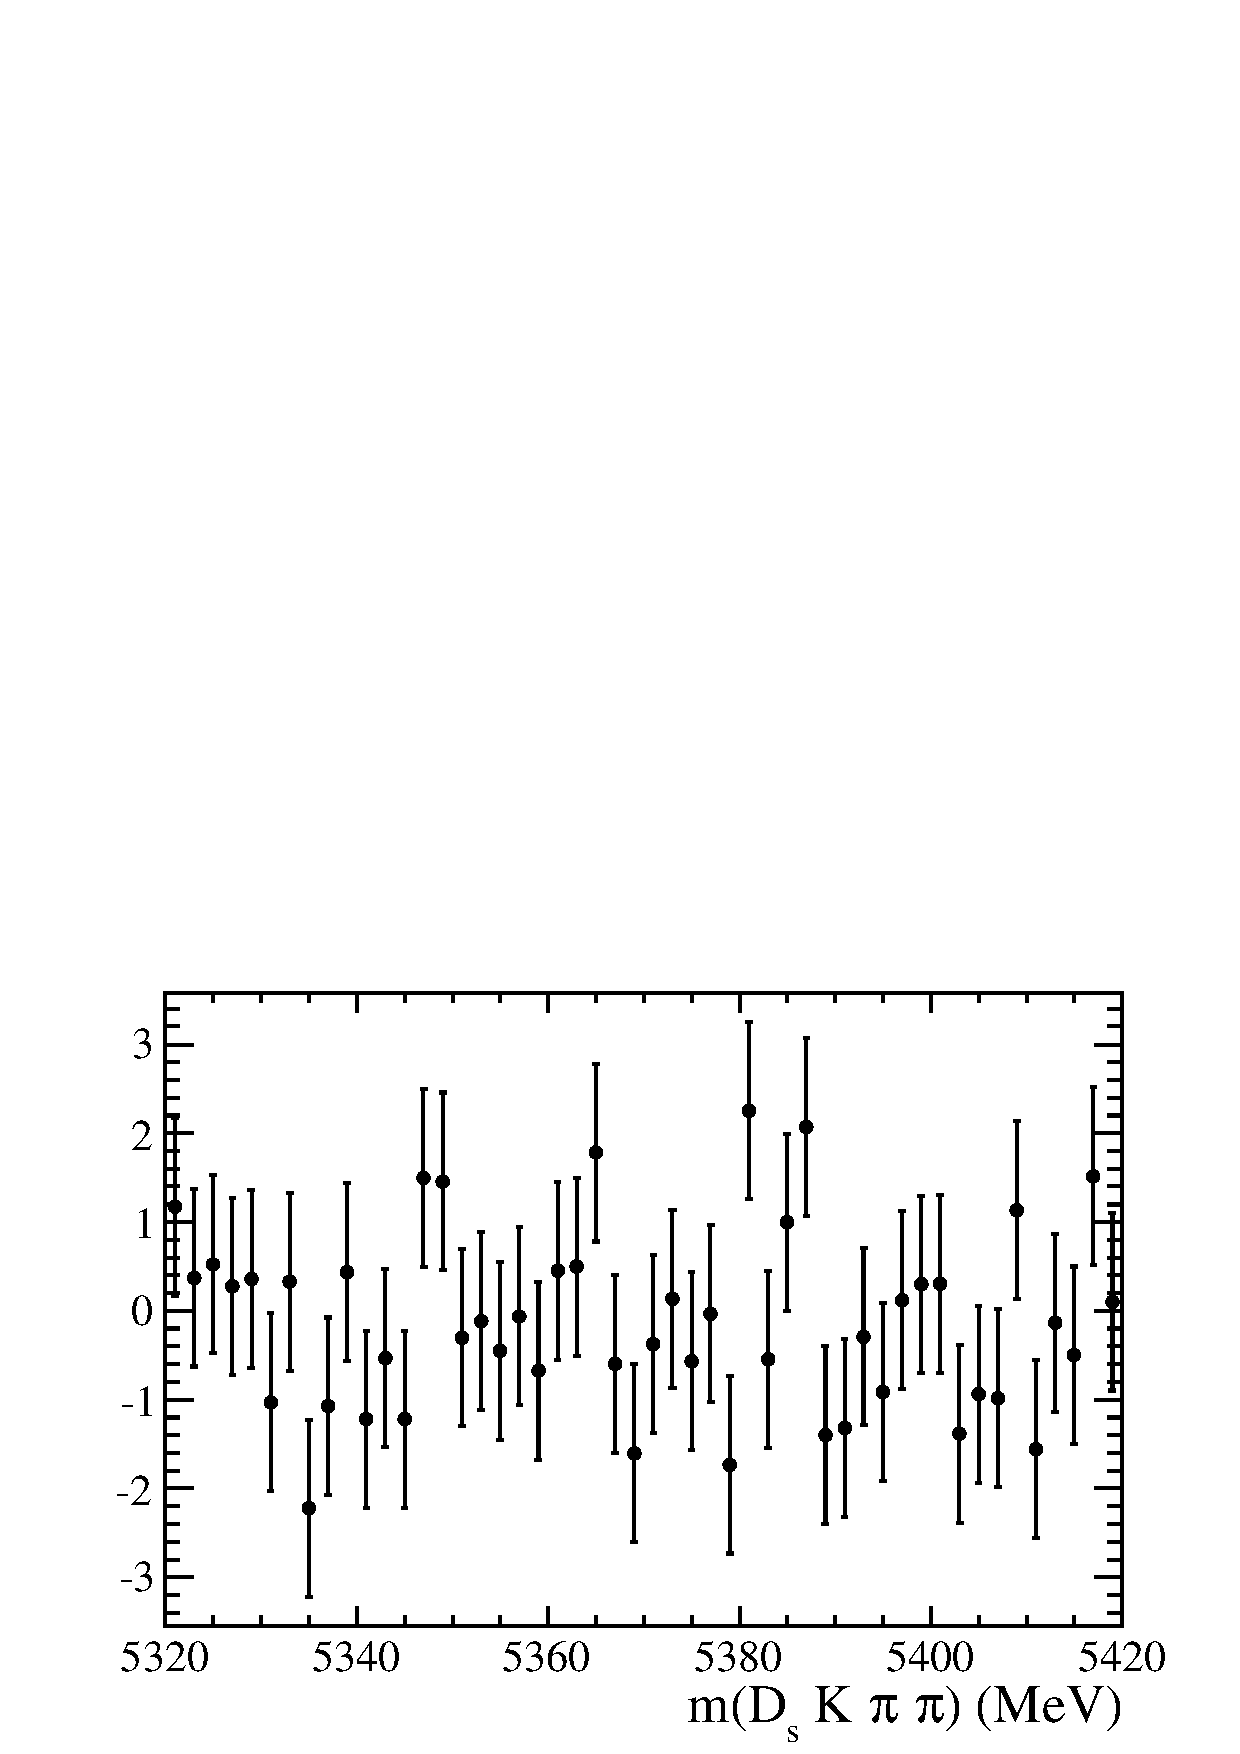
\includegraphics[height=!,width=0.45\textwidth]{figs/MassFit/normMC_pull.pdf} \hfill
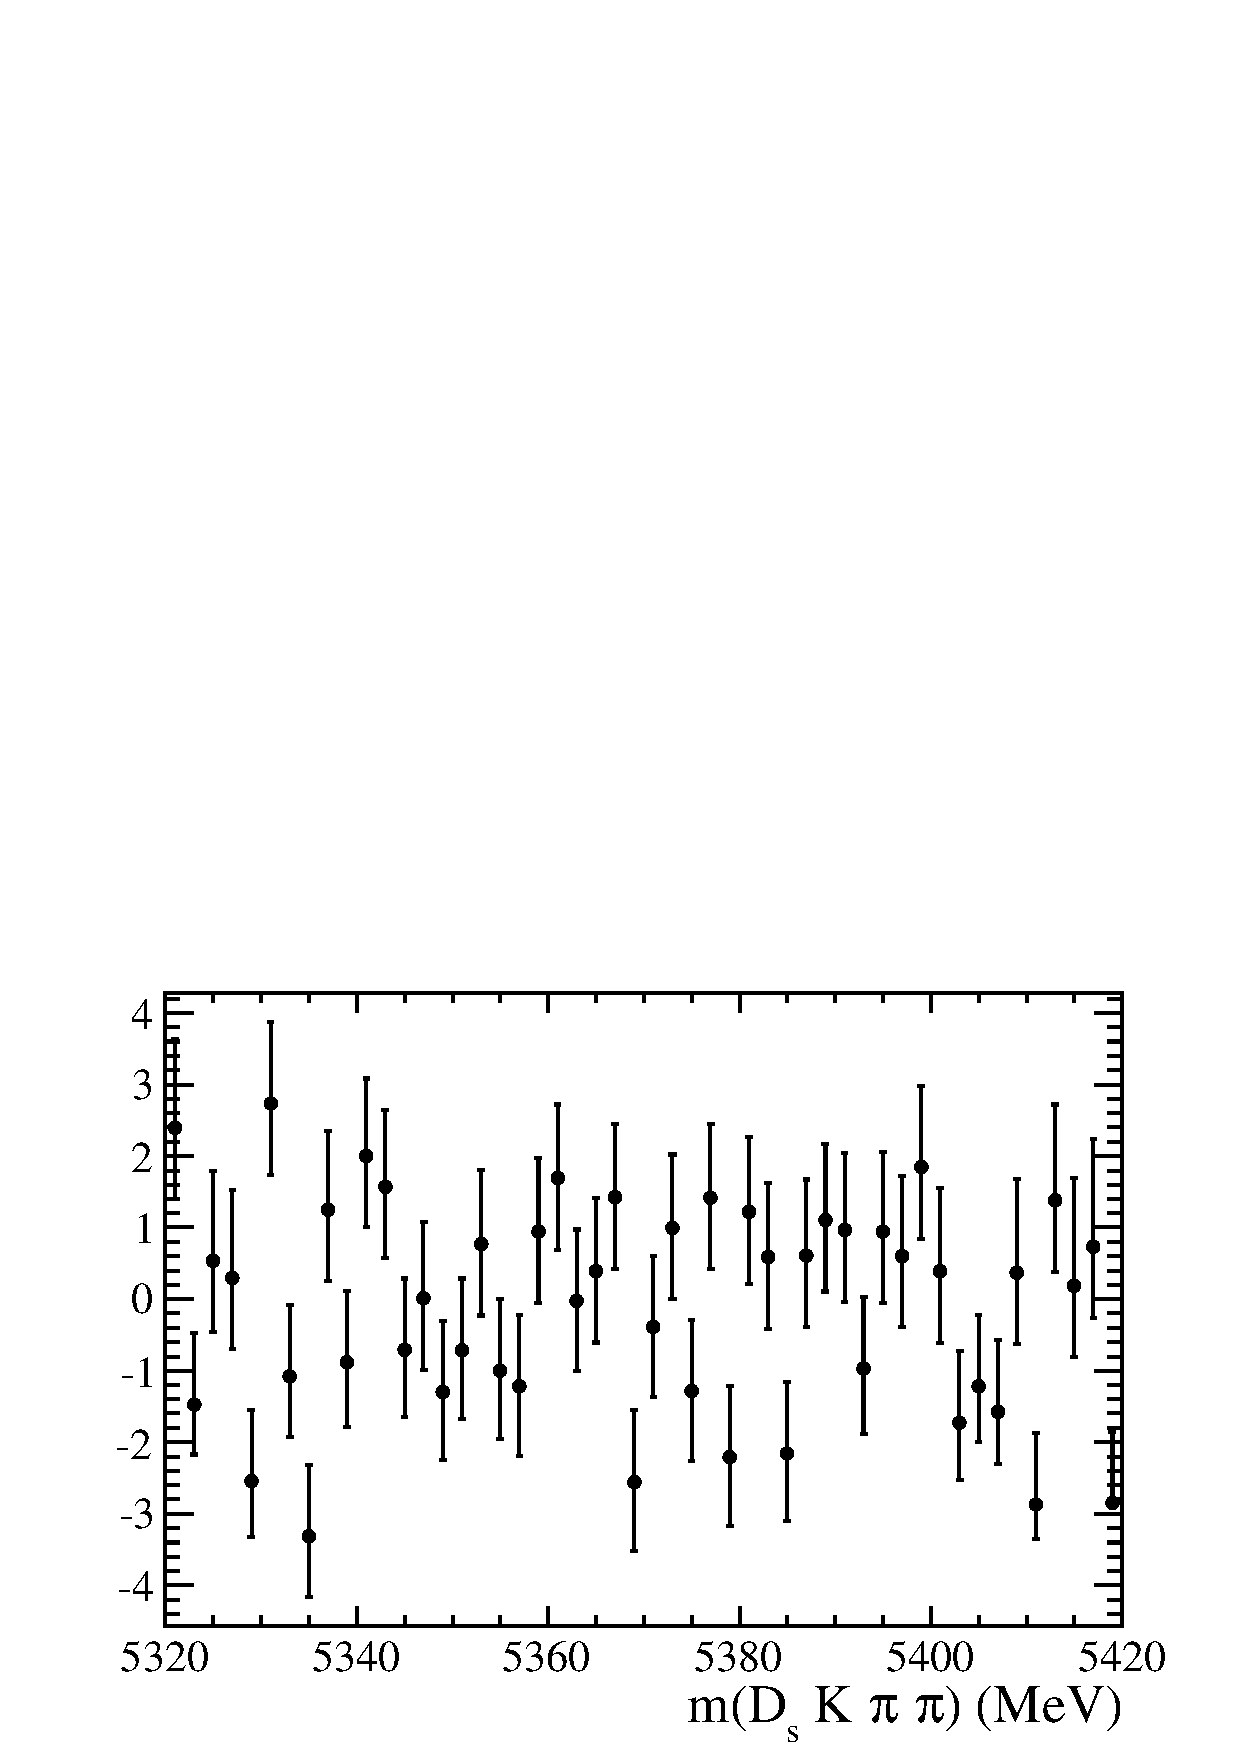
\includegraphics[height=!,width=0.45\textwidth]{figs/MassFit/signalMC_pull.pdf}
\caption{Invariant mass distributions of simulated (left) $\Bs\to\Ds\pion\pion\pion$ and (right) $\Bs\to\Ds\kaon\pion\pion$ events. A fit with a Johnson's SU PDF is overlaid.}
\label{fig: BsMassShapes}
\end{figure}
To account for differences between simulation and real data, linear scaling factors for the mean $\mu$ and width $\sigma$ are determined in the fit to $\Bs\to\Ds\pion\pion\pion$ data  
and later fixed in the fit to $\Bs\to\Ds\kaon\pion\pion$ decays. 
The scale factors are determined separately for each data-taking period and each trigger category.



\subsection{Background models} 
\label{subsec:bkgModel}

After the full selection we assume that the following residual background components have to be accounted for: \\
%\begin{itemize}
%
%	\item combinatorial background;%: This contribution arises from either a real $\Ds$, which is paired with random tracks to form the $\Bs$ candidates, or via real $X_{d}$'s, which are 	combined with three tracks that fake a $\Ds$ candidate to form a fake $\Bs$.   
%
%	\item peaking background from true $B^0 \to D_s h \pi \pi$ decays;
%
%	\item partially reconstructed $\Bz/\Bs\to D_s^{*}h\pion\pion$ decays, with $D_s^{*}\to\Ds\gamma$ or $D_s^{*}\to\Ds\piz$, where the $\gamma$/$\piz$ is not reconstructed;
%
%	\item misidentified $\Bs\to\Ds\pion\pion\pion$ decays, where one of the pions is wrongly identified as a kaon $\pion\rightarrow\kaon$; 
%
%	\item misidentified, partially reconstructed $\Bs\to D_s^{*}\pion\pion\pion$ decays, where one of the pions is wrongly identified as a kaon $\pion\rightarrow\kaon$ and the $\gamma$/$\piz$ from $D_s^{*}\to\Ds\gamma$/$\piz$ is not reconstructed.
%
%\end{itemize}

\noindent \textbf{Combinatorial background}  \\
The combinatorial background is described by a second order polynomial,
whose parameters are determined, for each $D_s$ final state separately, in the fit to data.
%For systematic studies an exponential PDF is used.
\\

\noindent\textbf{Peaking $B_d$ background}  \\
Decays of $B_d$ mesons into the $D_s h \pi \pi$ final state are described by the $B_s$ signal PDF where the mean is shifted by the known mass difference $m_{B_s} - m_{B_d}$\cite{Agashe:2014kda}.
\\

\noindent \textbf{Partially reconstructed background}  \\
The shape of the  $\Bs\to D_s^{*}\pion\pion\pion$ contribution is expected to be peaking in the $m(\Ds\pion\pion\pion)$ spectrum, with large tails due to the missing momentum, which is carried away by the $\piz$ or $\gamma$. 
%The pion or photon from $\Ds^{*}\to\Ds(\gamma/\piz)$ is excluded from the reconstruction. 
We model the shape of this contribution using the sum of three bifurcated Gaussian functions.
Figure \ref{fig: BsDsstar3piMC} shows the fit of the sum of three bifurcated Gaussian functions to the invariant mass distribution of simulated $\Bs\to D_s^{*}\pion\pion\pion$ event. 
The shape parameters, 
%are used as input values for the nominal $m(\Ds\pion\pion\pion)$ mass fit. 
as well as the yield of this contribution, are directly determined on data from a fit to the $m(\Ds\pion\pion\pion)$ invariant mass distribution. 
For the contribution of the $\Bz\to D_s^{*}\kaon\pion\pion$ background, the same shape is used but the means $\mu_{i}$ of the bifurcated gaussians are shifted down by $m_{\Bs} - m_{\Bz}$ \cite{Agashe:2014kda}. 
The yields of both contributions are directly determined in the nominal fit. \\

\noindent\textbf{Miss-identified background}  \\
To determine the shape of misidentified $\Bs\to\Ds\pion\pion\pion$ candidates in the $m(\Ds\kaon\pion\pion)$ spectrum, we take a truth-matched signal MC sample of our normalization channel. 
We then use the PIDCalib package to determine the $\pion\rightarrow\kaon$ fake rate. For every candidate in our MC sample, a (momentum) $\ptot$ and (pseudorapidity) $\eta$-dependent event weight is computed and assigned. 
We flip the particle hypothesis from pion to kaon for the $\pion$ with the biggest miss-ID weight for each event and recompute the invariant $\Bs$ mass. This distribution is then modeled using two Crystal Ball functions. 
The distribution and the fit are shown in Fig. \ref{fig: BsDspipipiMCmissID}(left). 

The expected yield of misidentified $\Bs\to\Ds\pion\pion\pion$ candidates in the $m(\Ds\kaon\pion\pion)$ spectrum is computed by multiplying the fake probability of $\propto3.2\%$, which is derived from PIDCalib, by the yield of $\Bs\to\Ds\pion\pion\pion$ signal candidates, determined in the nominal mass fit of our normalization channel.  \newline
In the same way as mentioned above, we can determine the rate of misidentified, partially reconstructed $\Bs\to\Ds^{*}\pion\pion\pion$ decays in our sample of $\Bs\to\Ds\kaon\pion\pion$ decays using PIDCalib and a MC sample of $\Bs\to\Ds^{*}\pion\pion\pion$ events. The invariant mass distribution we obtain when we exclude the $\gamma$/$\piz$, flip the the particle hypothesis $\pion\rightarrow\kaon$ and apply the event weights given by the fake rate, is shown in Fig. \ref{fig: BsDspipipiMCmissID} (right). The fit of two Crystal Ball functions to this distribution is overlaid. 
The yield of this contribution is determined from the yield of $\Bs\to\Ds^{*}\pion\pion\pion$ candidates in the nominal mass fit of our normalization channel, multiplied by the misID probability of $\propto 3.6\%$.

%
%\begin{figure}[h]
%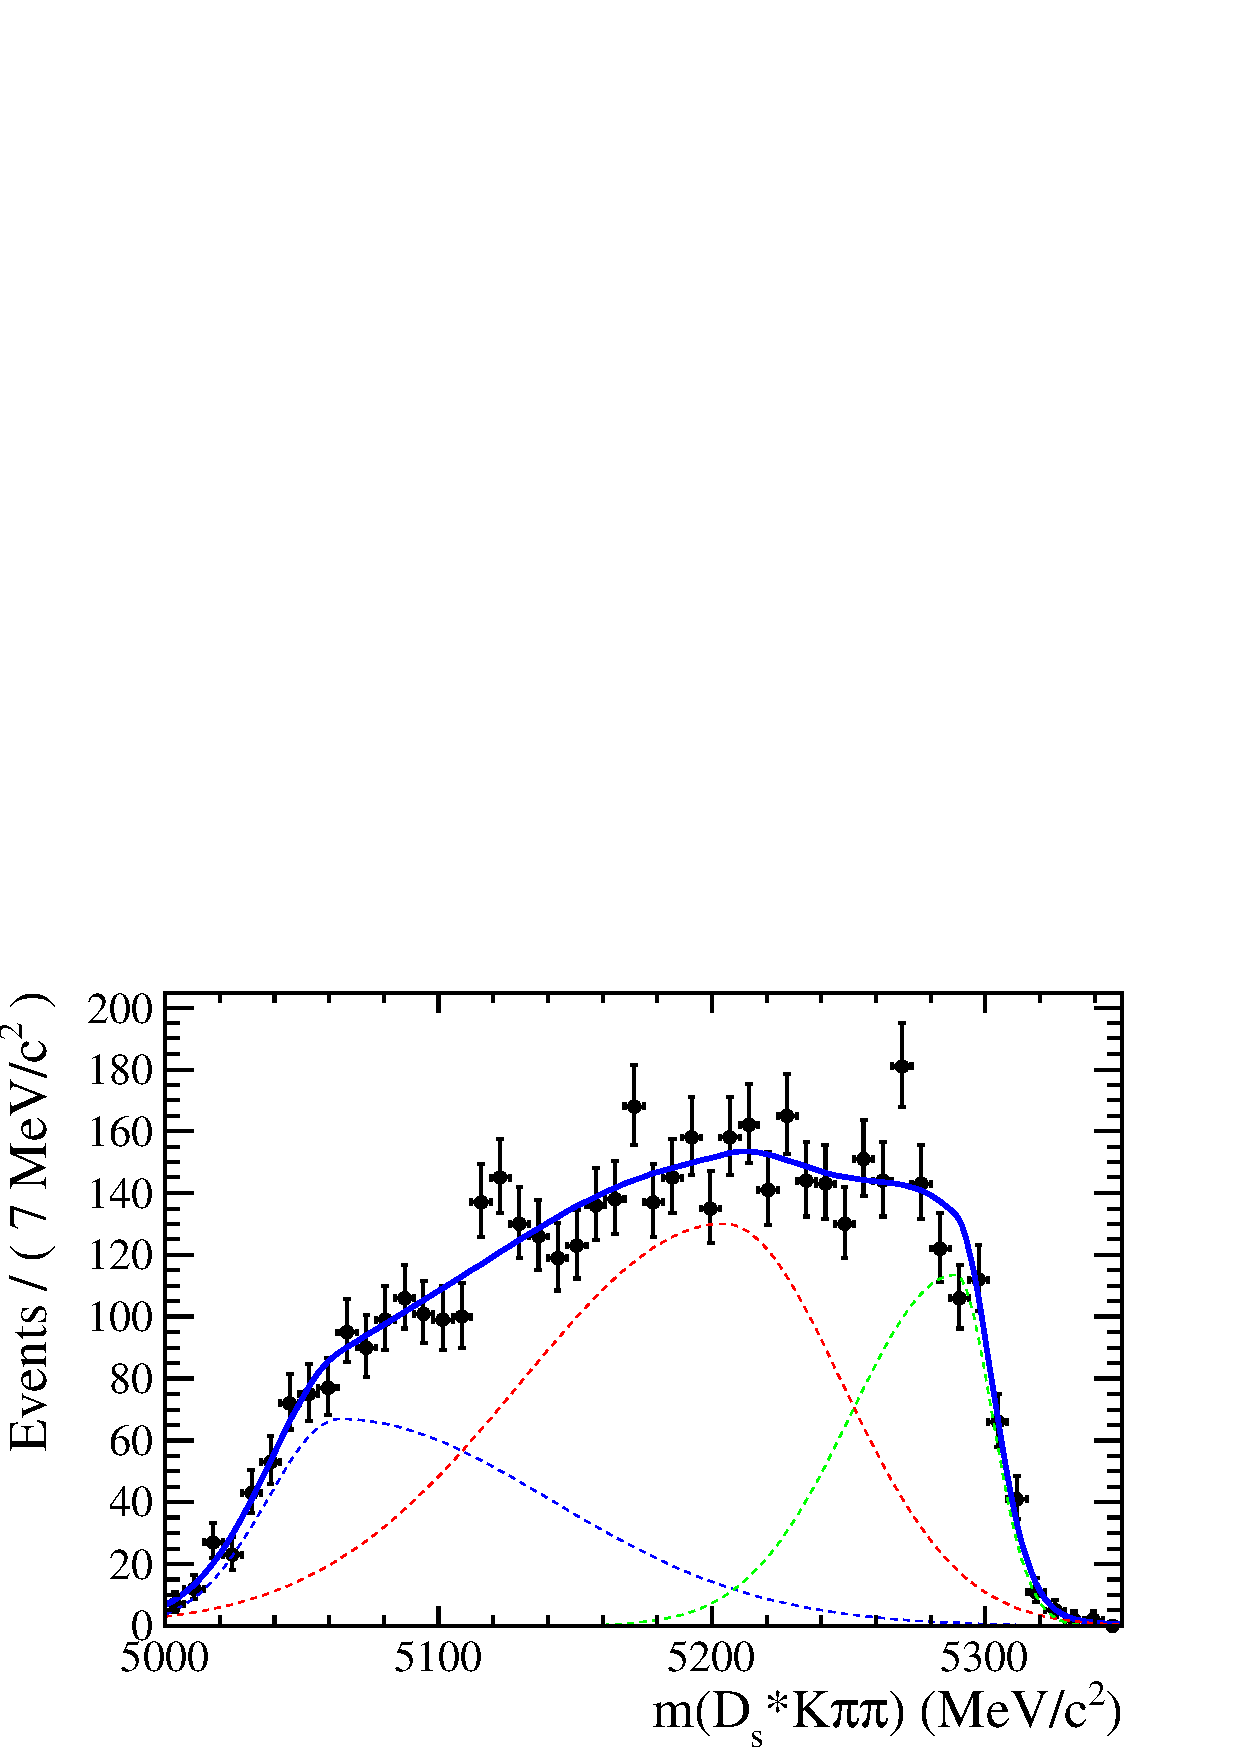
\includegraphics[height=!,width=0.4\textwidth]{figs/Bs2Dsstartpipipi.pdf}
%\caption{Invariant mass distribution of simulated $\Bs\to\Ds^{*}\pion\pion\pion$ events, where the $\gamma$/$\piz$ is excluded from the reconstruction. 
%A fit of the sum of three bifurcated Gaussian functions to this distribution is overlaid.}
%\label{fig: BsDsstar3piMC}
%\end{figure}

\begin{figure}[h]
\centering
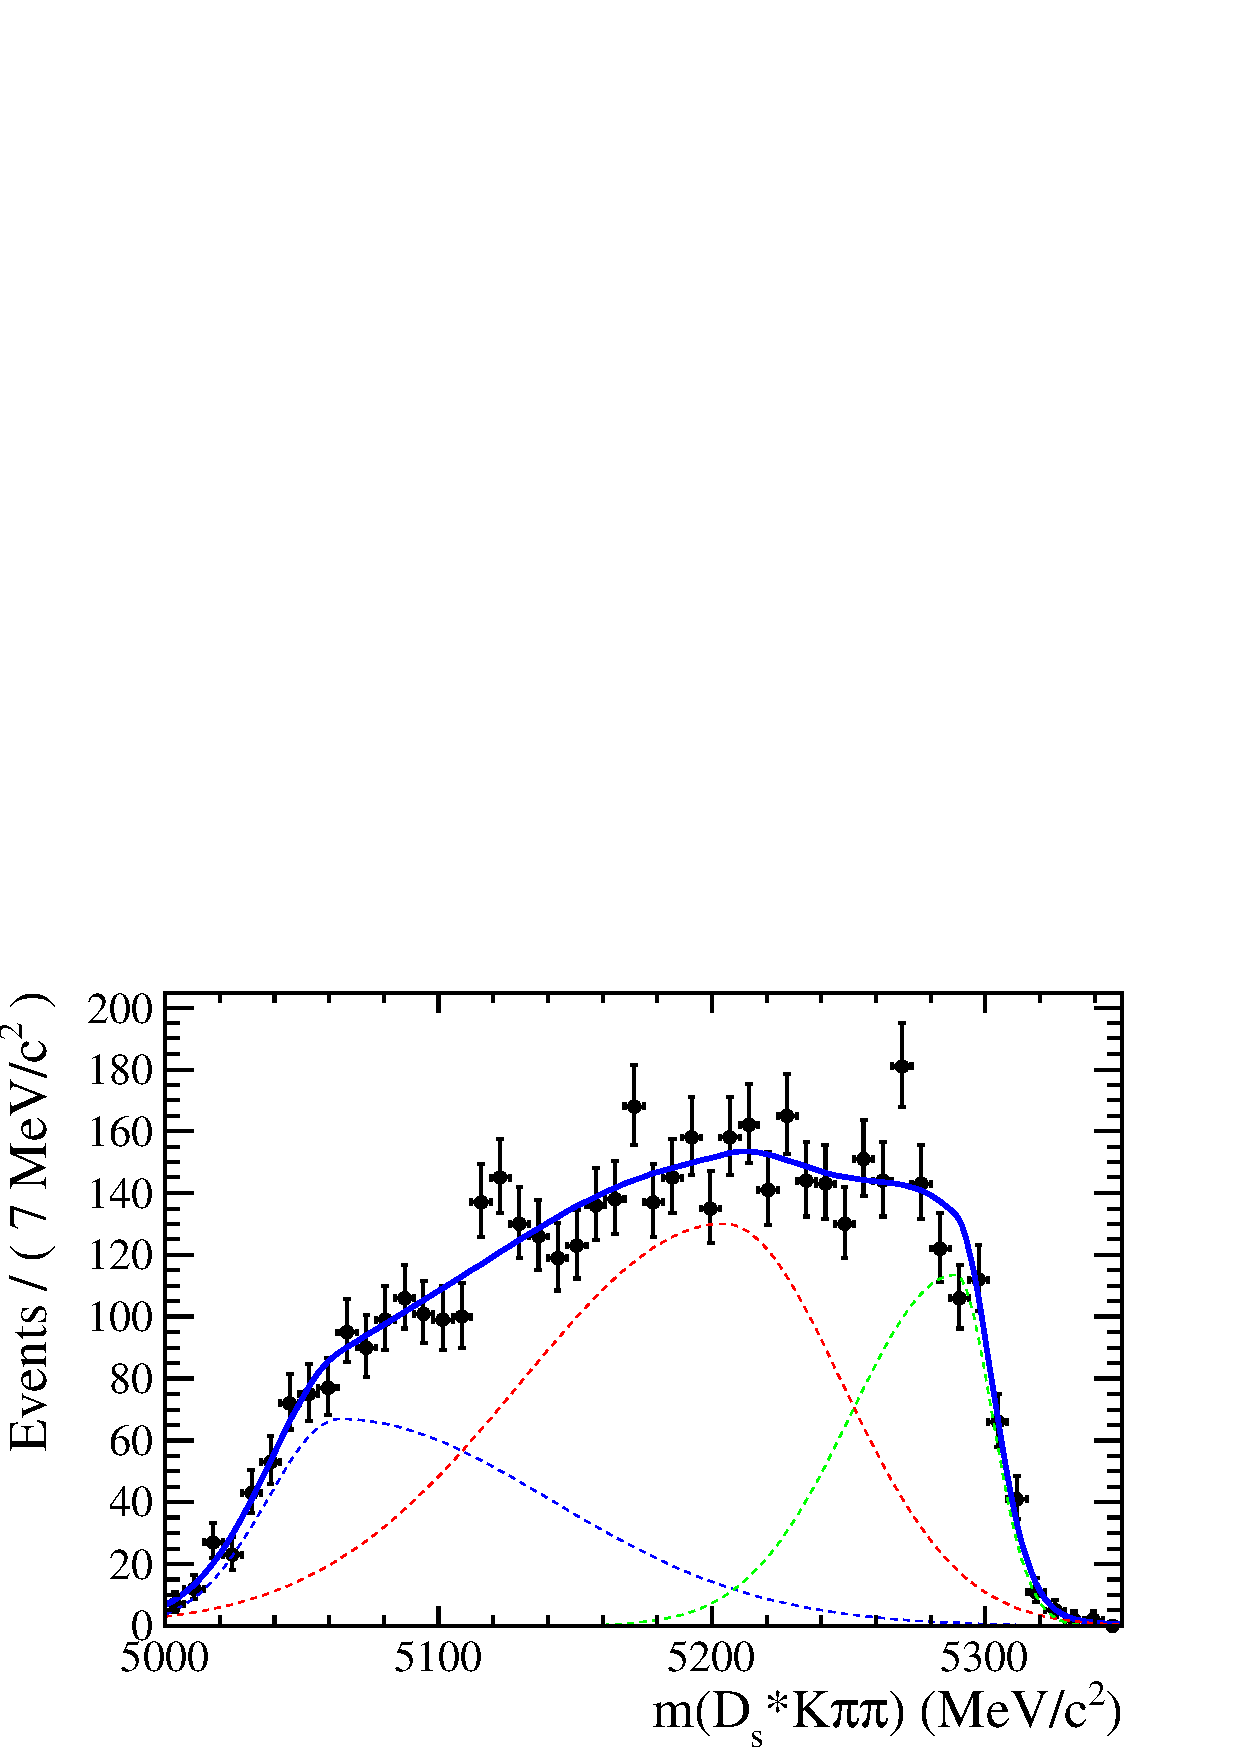
\includegraphics[height=!,width=0.32\textwidth]{figs/Bs2Dsstartpipipi.pdf}
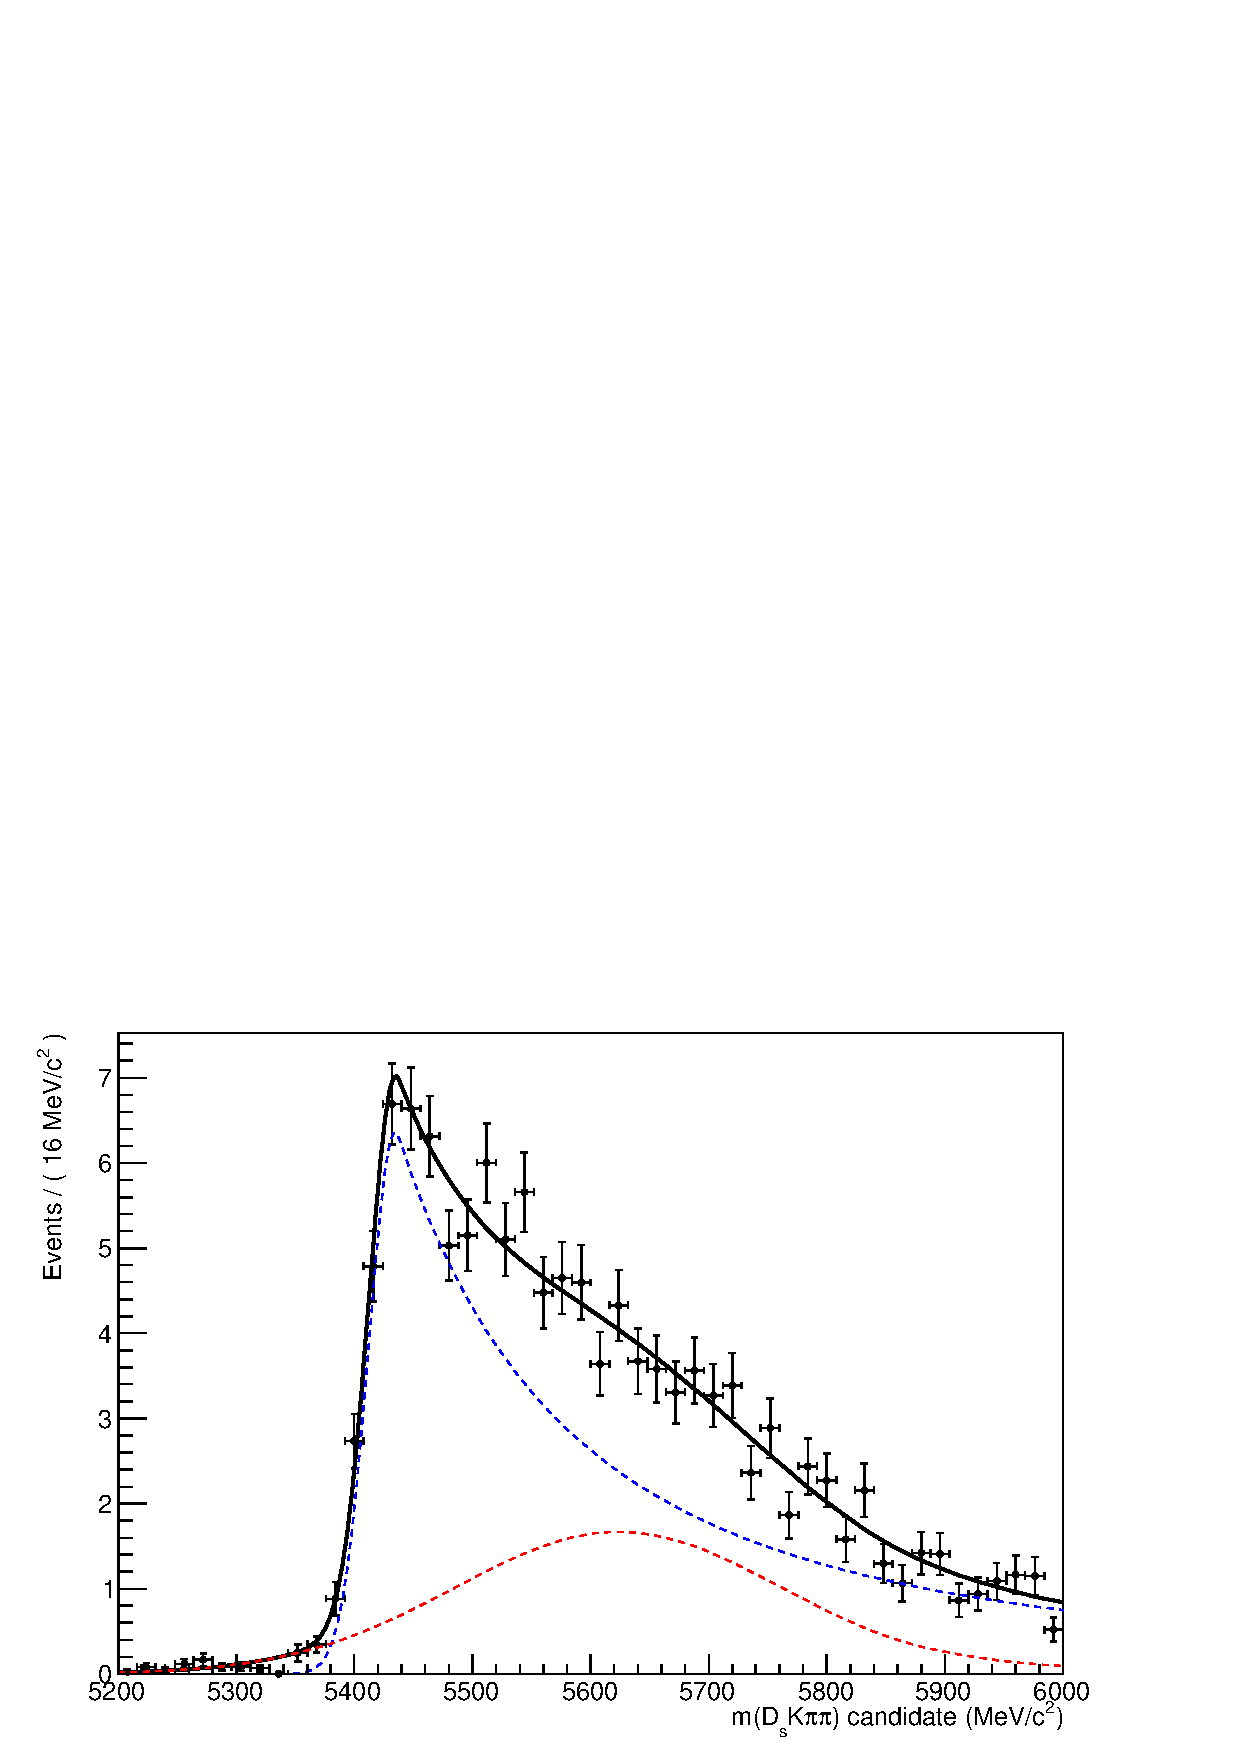
\includegraphics[height=!,width=0.32\textwidth]{figs/Bs2Dspipipi_as_DsKpipi.pdf}
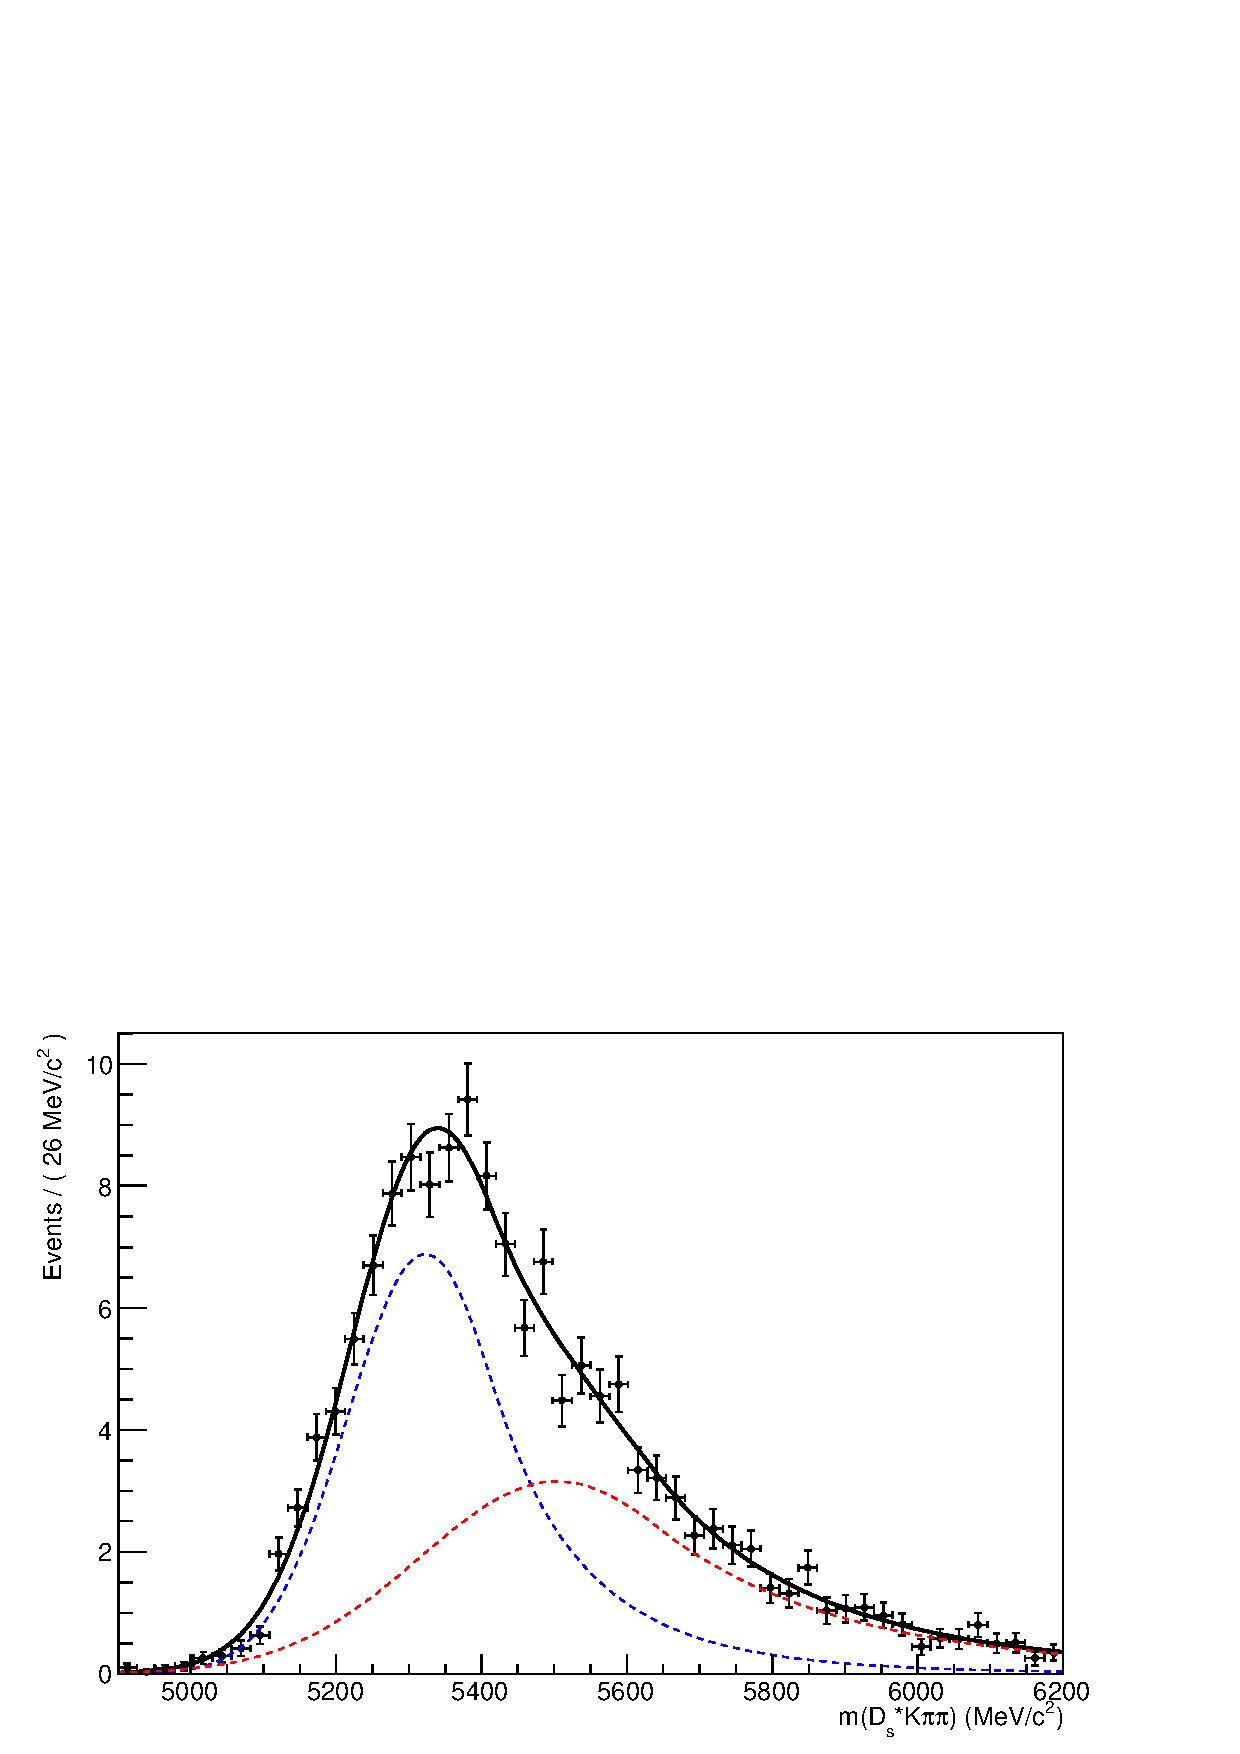
\includegraphics[height=!,width=0.32\textwidth]{figs/Bs2Dsstarpipipi_as_DsKpipi.pdf}
\caption{
Left: Invariant mass distribution of simulated $\Bs\to D_s^{*}\pion\pion\pion$ events, where the $\gamma$/$\piz$ is excluded from the reconstruction. 
Middle: Invariant mass distribution of  simulated $\Bs\to\Ds\pion\pion\pion$ events, where one of the pions is reconstructed as a kaon taking the misID probability into account. 
Right: Invariant mass distribution for simulated $\Bs\to D_s^{*}\pion\pion\pion$ events, where the $\gamma$/$\piz$ from the $D_s^{*}$ is excluded from reconstruction
and one of the pions is reconstructed as a kaon taking the misID probability into account. The fitted PDF is shown in blue.}
\label{fig: BsDspipipiMCmissID}
\end{figure}
 

%\subsection{Fit to $\Bs\to\Ds\pion\pion\pion$ candidates}
%\label{subsec: NormFit}
%
%An unbinned maximum likelihood fit is performed simultaneously to the invariant mass distribution of $\Bs\to\Ds\pion\pion\pion$ candidates. 
%As discussed in Sec. \ref{subsec: signalmodel}, the fit is given as a Johnson SU signal model for the $\Bs$ and $\Bz$ signal, the sum of three bifurcated Gaussian functions to model the partially reconstructed $\Bs\to\Ds^{*}\pion\pion\pion$ background and an Exponential function to account for combinatorial background. The invariant mass distribution and the fit is shown in Fig.~\ref{fig: BsDsKpipiFit}. 
%All simultaneously performed fits to the $m(\Ds\pion\pion\pion)$ distribution, ordered by the respective $\Ds$ final state, can be found in the Appendix \ref{subsec:DetailedMassfits}.   
%The obtained yields are summarized in Table \ref{table:YieldsFromMassfit}. 
%
%
%\subsection{Fit to $\Bs\to\Ds\kaon\pion\pion$ candidates}
%\label{subsec: SigFit}
%
%The shape of the invariant mass distribution of$\Bs\to\Ds\kaon\pion\pion$ candidates is described by Johnson SU functions for the $\Bz$ and $\Bs$ signal, 
%two sums of three bifurcated Gaussians for the $\Bs$/$\Bz\to\Ds^{*}\kaon\pion\pion$ partially reconstructed background contributions and 
%two sums of double Crystal Ball functions for the single misID $\Bs\to\Ds\pion\pion\pion$ and the partially reconstructed, misidentified $\Bs\to\Ds^{*}\pion\pion\pion$ decays. 
%A simultaneous unbinned maximum likelihood fit is performed and the result is shown in Fig.~\ref{fig: BsDsKpipiFit}.
%All simultaneously performed fits to the $m(\Ds\kaon\pion\pion)$ distribution, ordered by the respective $\Ds$ final state, can be found in the Appendix \ref{subsec:DetailedMassfits}.
%The obtained yields are summarized in Table \ref{table:YieldsFromMassfit}.
% 

\subsection{Results}
\label{subsec:Results}

The sPlot technique \cite{Pivk:2004ty} is used to extract signal weights from the fits to the invariant mass distributions of our signal and normalizaton channel. 
This statistical tool assignes a weight to every event, according to it's position in the respective mass distribution, given the fitted signal and background models. 
The weights can then be used to suppress the background components in every other observable distribution of interest.  
Figure \ref{fig: sWeights} shows the distribution of weights across the invariant mass spectra of $\Bs\to\Ds\pion\pion\pion$ and $\Bs\to\Ds\kaon\pion\pion$ candidates.


\begin{figure}[h]
\centering
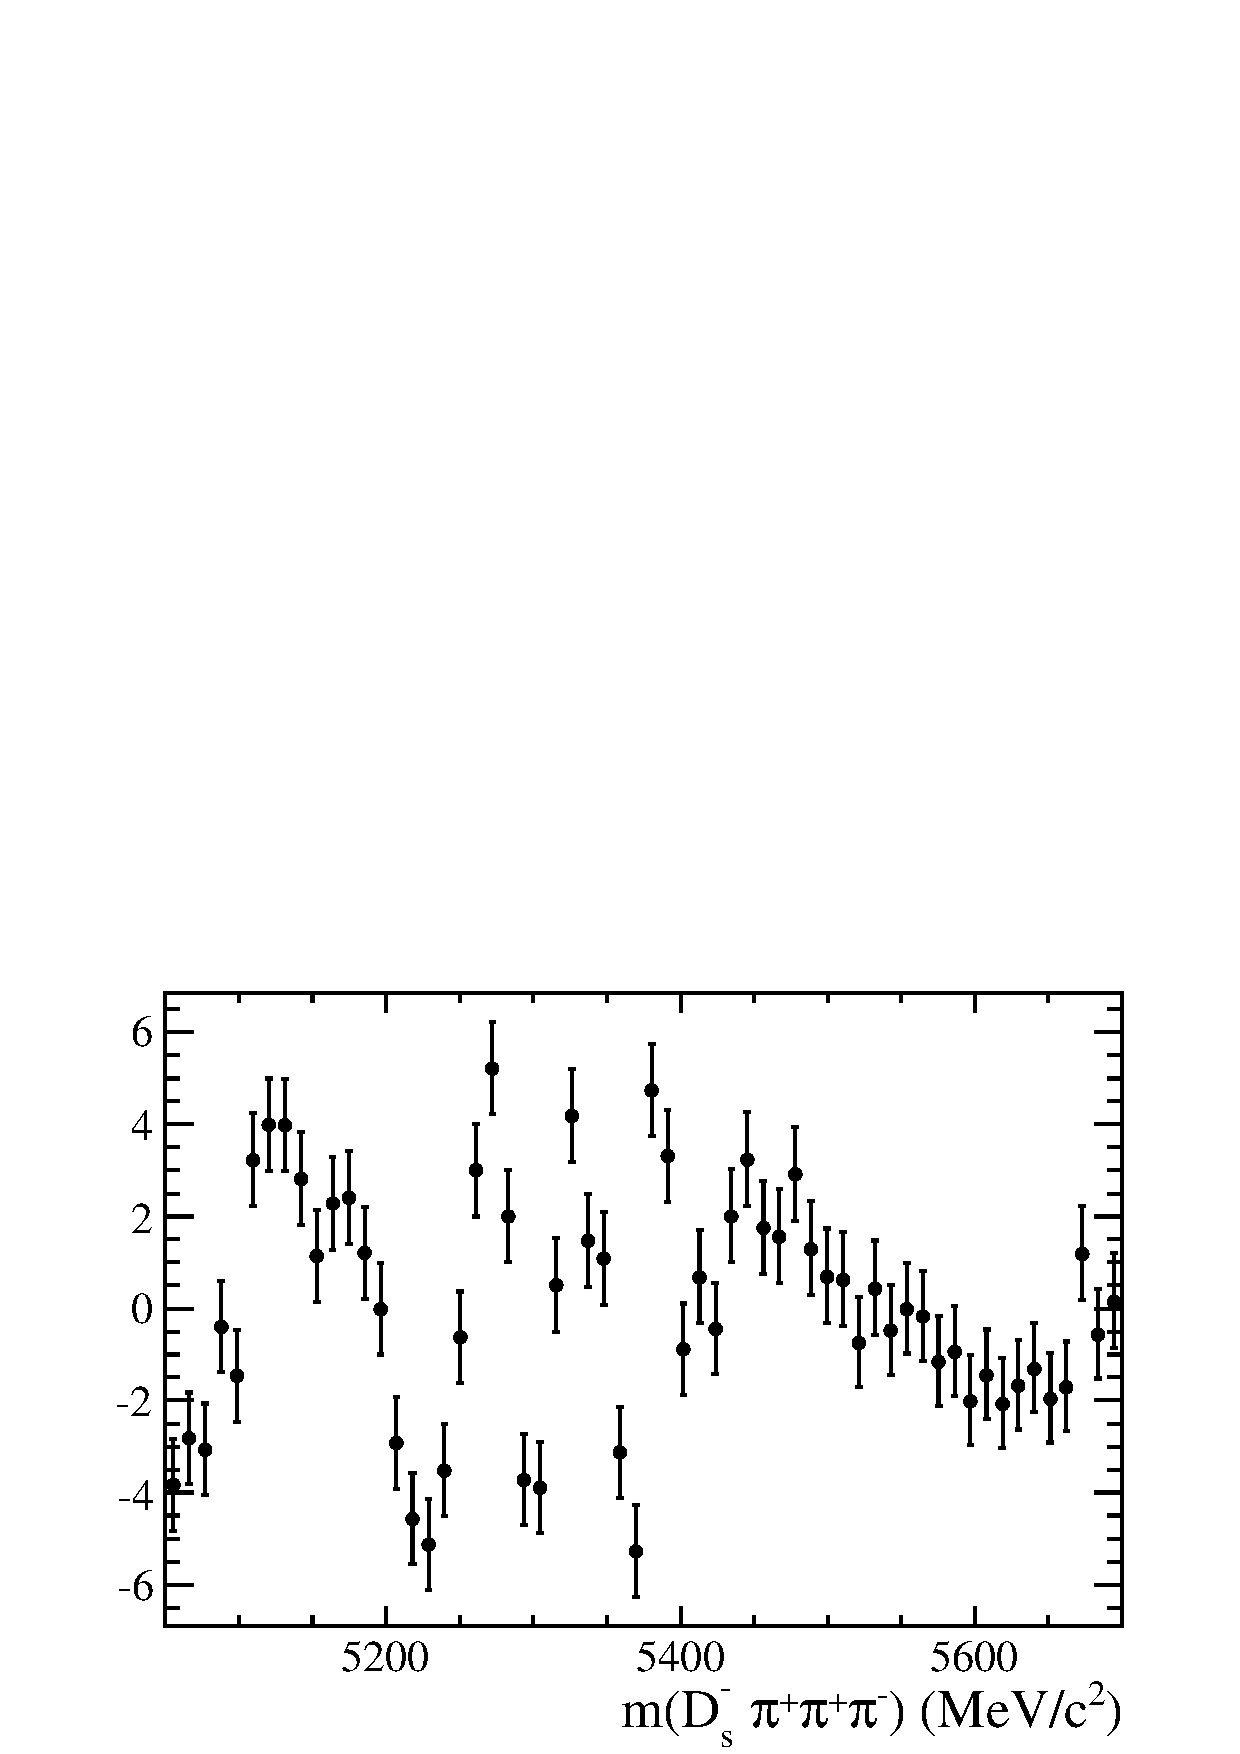
\includegraphics[height=!,width=0.49\textwidth]{figs/MassFit/norm_pull.pdf}
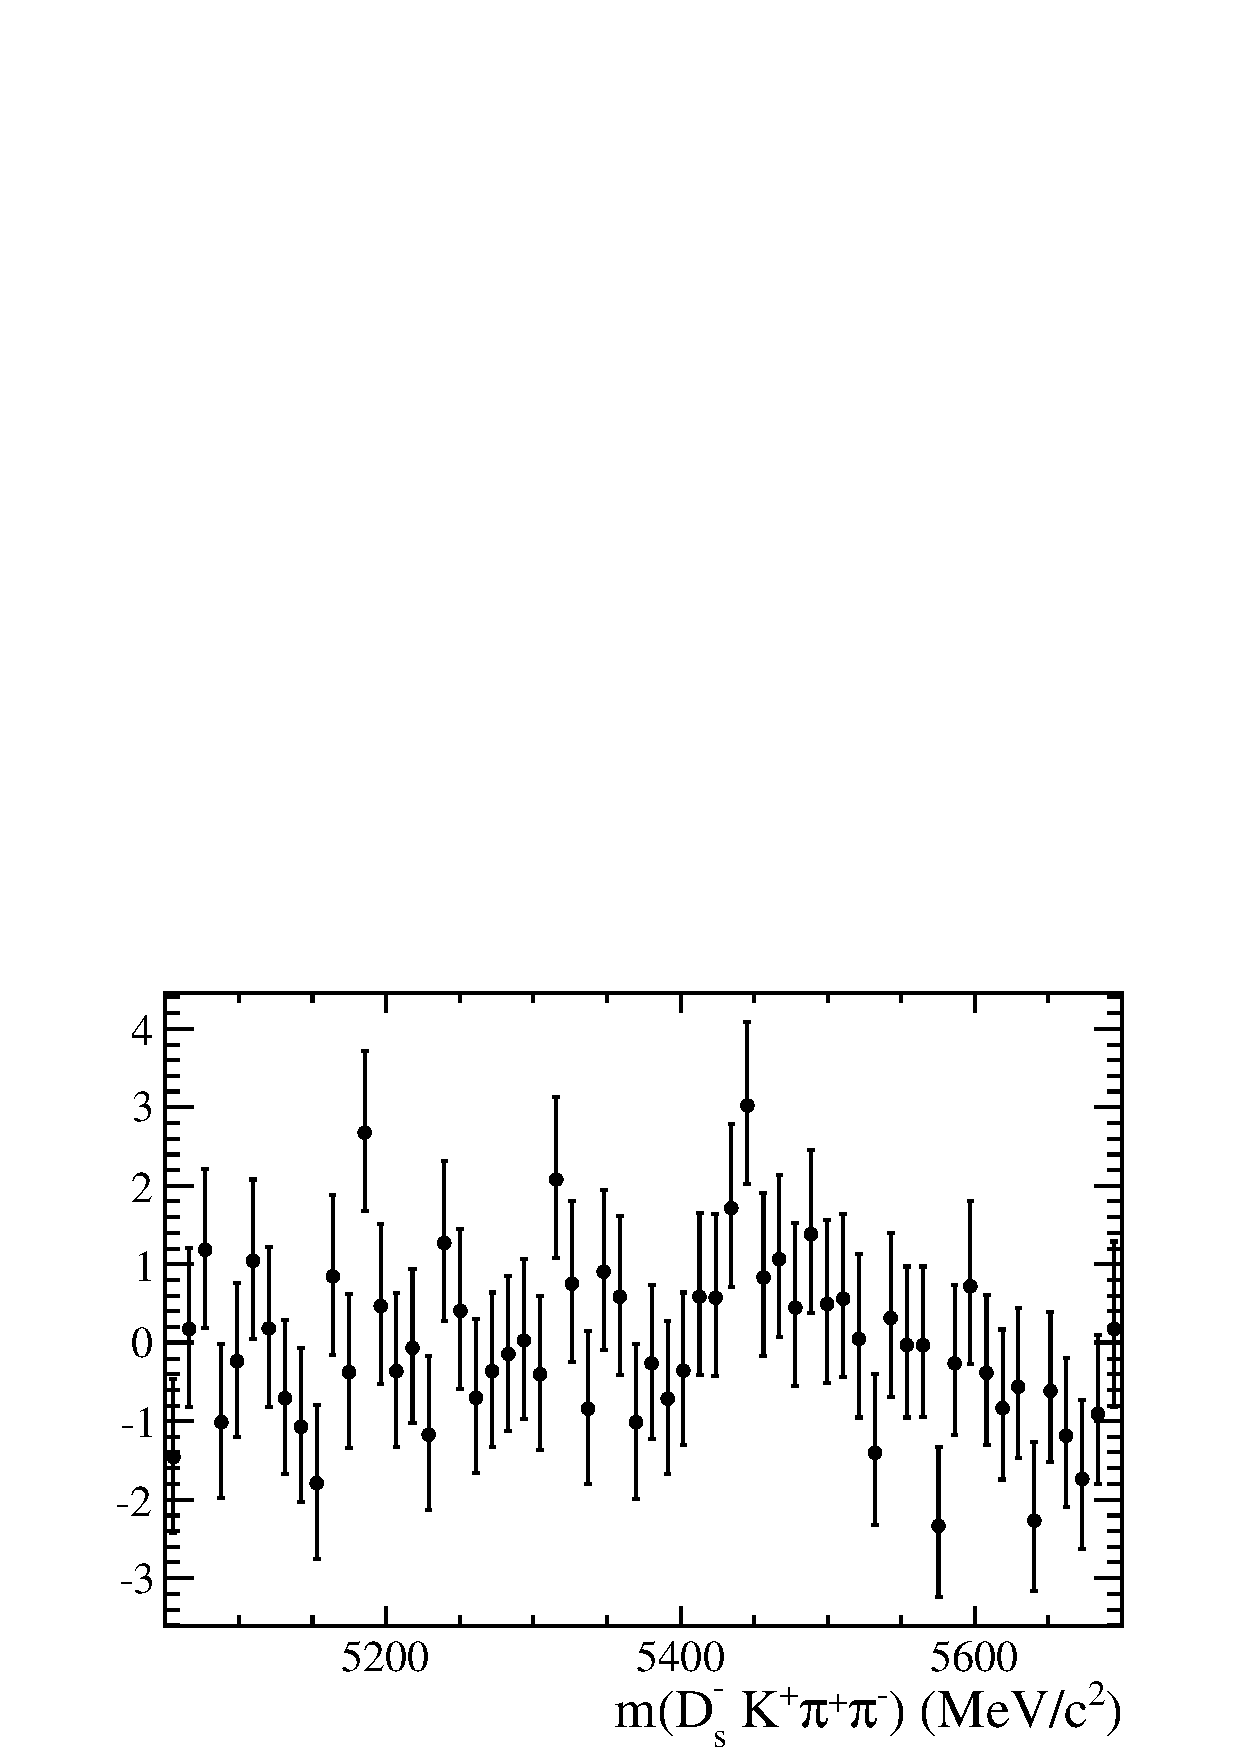
\includegraphics[height=!,width=0.49\textwidth]{figs/MassFit/signal_pull.pdf}
\caption{Invariant mass distribution of (left) $\Bs\to\Ds\pion\pion\pion$ and (right) $\Bs\to\Ds\kaon\pion\pion$ candidates for Run-I and Run-II data.
The respective fit described in the text is overlaid.}
\label{fig: BsDsKpipiFit}
\end{figure}


\begin{table}[h]
\centering
 \begin{tabular}{l || l l l l}
fit component & yield 2011 & yield 2012 & yield 2015 & yield 2016\ \\
\hline\hline
$m(\Ds\kaon\pion\pion)$ &  &  &  &  \\
\hline
$\Bs\to\Ds\kaon\pion\pion$ & 392 $\pm$ 25 & 860 $\pm$ 38 & 309 $\pm$ 21 & 1984 $\pm$ 55 \\
$\Bz\to\Ds\kaon\pion\pion$ & 276 $\pm$ 26 & 692 $\pm$ 41 & 261 $\pm$ 23 & 1385 $\pm$ 58 \\
$\Bz/\Bs\to\Ds^{*}\kaon\pion\pion$ & 7 $\pm$ 25 & 171 $\pm$ 75 & 114 $\pm$ 25 & 893 $\pm$ 84 \\
$\Bs\to\Ds^{(*)}\pion\pion\pion$ & 63 $\pm$ 0 & 158 $\pm$ 0 & 53 $\pm$ 0 & 314 $\pm$ 0 \\
combinatorial & 1482 $\pm$ 53 & 2884 $\pm$ 100 & 605 $\pm$ 43 & 4261 $\pm$ 133 \\
\hline\hline
$m(\Ds\pion\pion\pion)$ &  &  &  &  \\
\hline
$\Bs\to\Ds\pion\pion\pion$ & 9183 $\pm$ 105 & 22083 $\pm$ 166 & 7574 $\pm$ 95 & 43773 $\pm$ 245 \\
$\Bz\to\Ds\pion\pion\pion$ & 289 $\pm$ 58 & 716 $\pm$ 95 & 229 $\pm$ 54 & 968 $\pm$ 147 \\
$\Bs\to\Ds^{*}\pion\pion\pion$ & 3640 $\pm$ 130 & 9086 $\pm$ 232 & 3047 $\pm$ 110 & 17827 $\pm$ 421 \\
combinatorial & 4991 $\pm$ 154 & 11127 $\pm$ 271 & 3728 $\pm$ 126 & 24589 $\pm$ 500 \\
\hline
\end{tabular}
\caption{Summary of yields obtained from the fits to Run1 and Run2 data.}
\label{table:YieldsFromMassfit}
\end{table}


%\begin{figure}[h]
%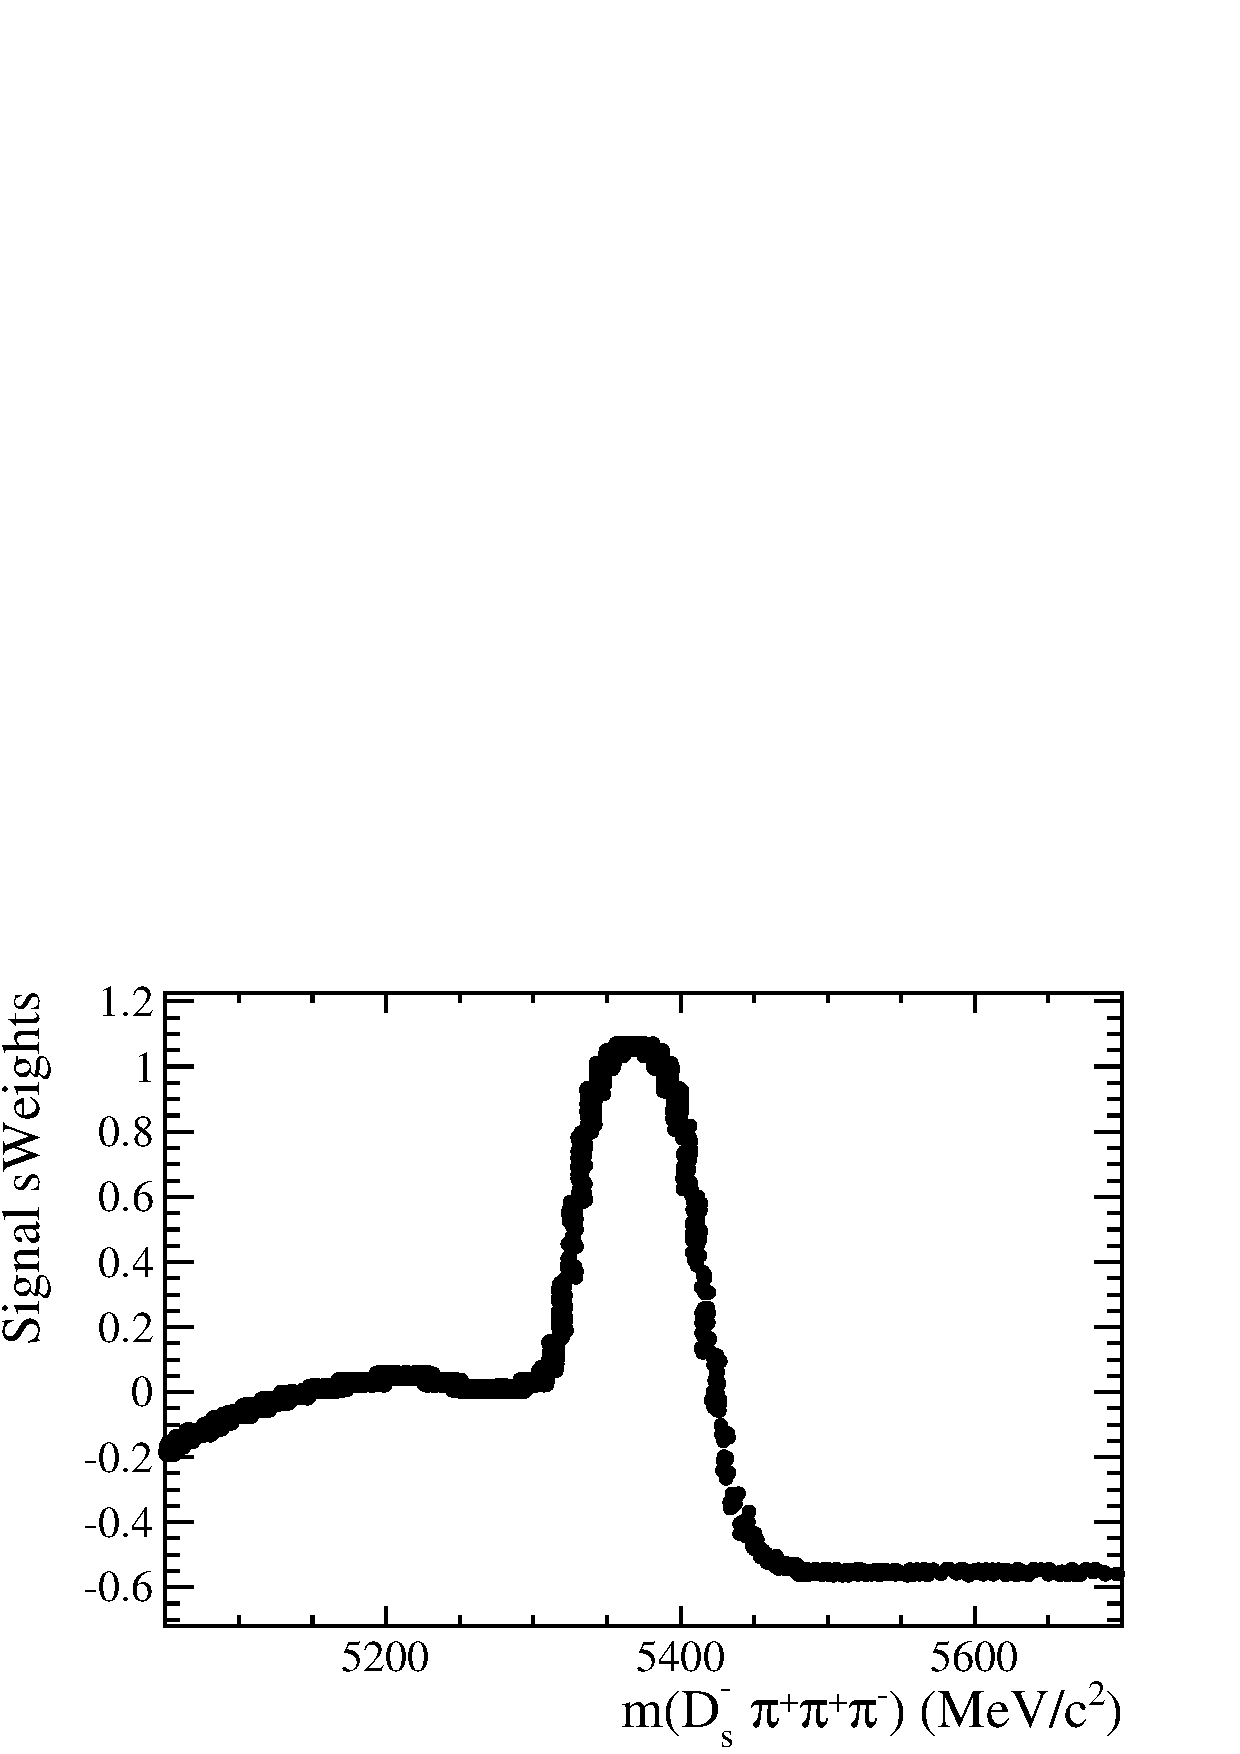
\includegraphics[height=7.cm,width=0.49\textwidth]{figs/norm_sweight_y11_phipi.pdf}
%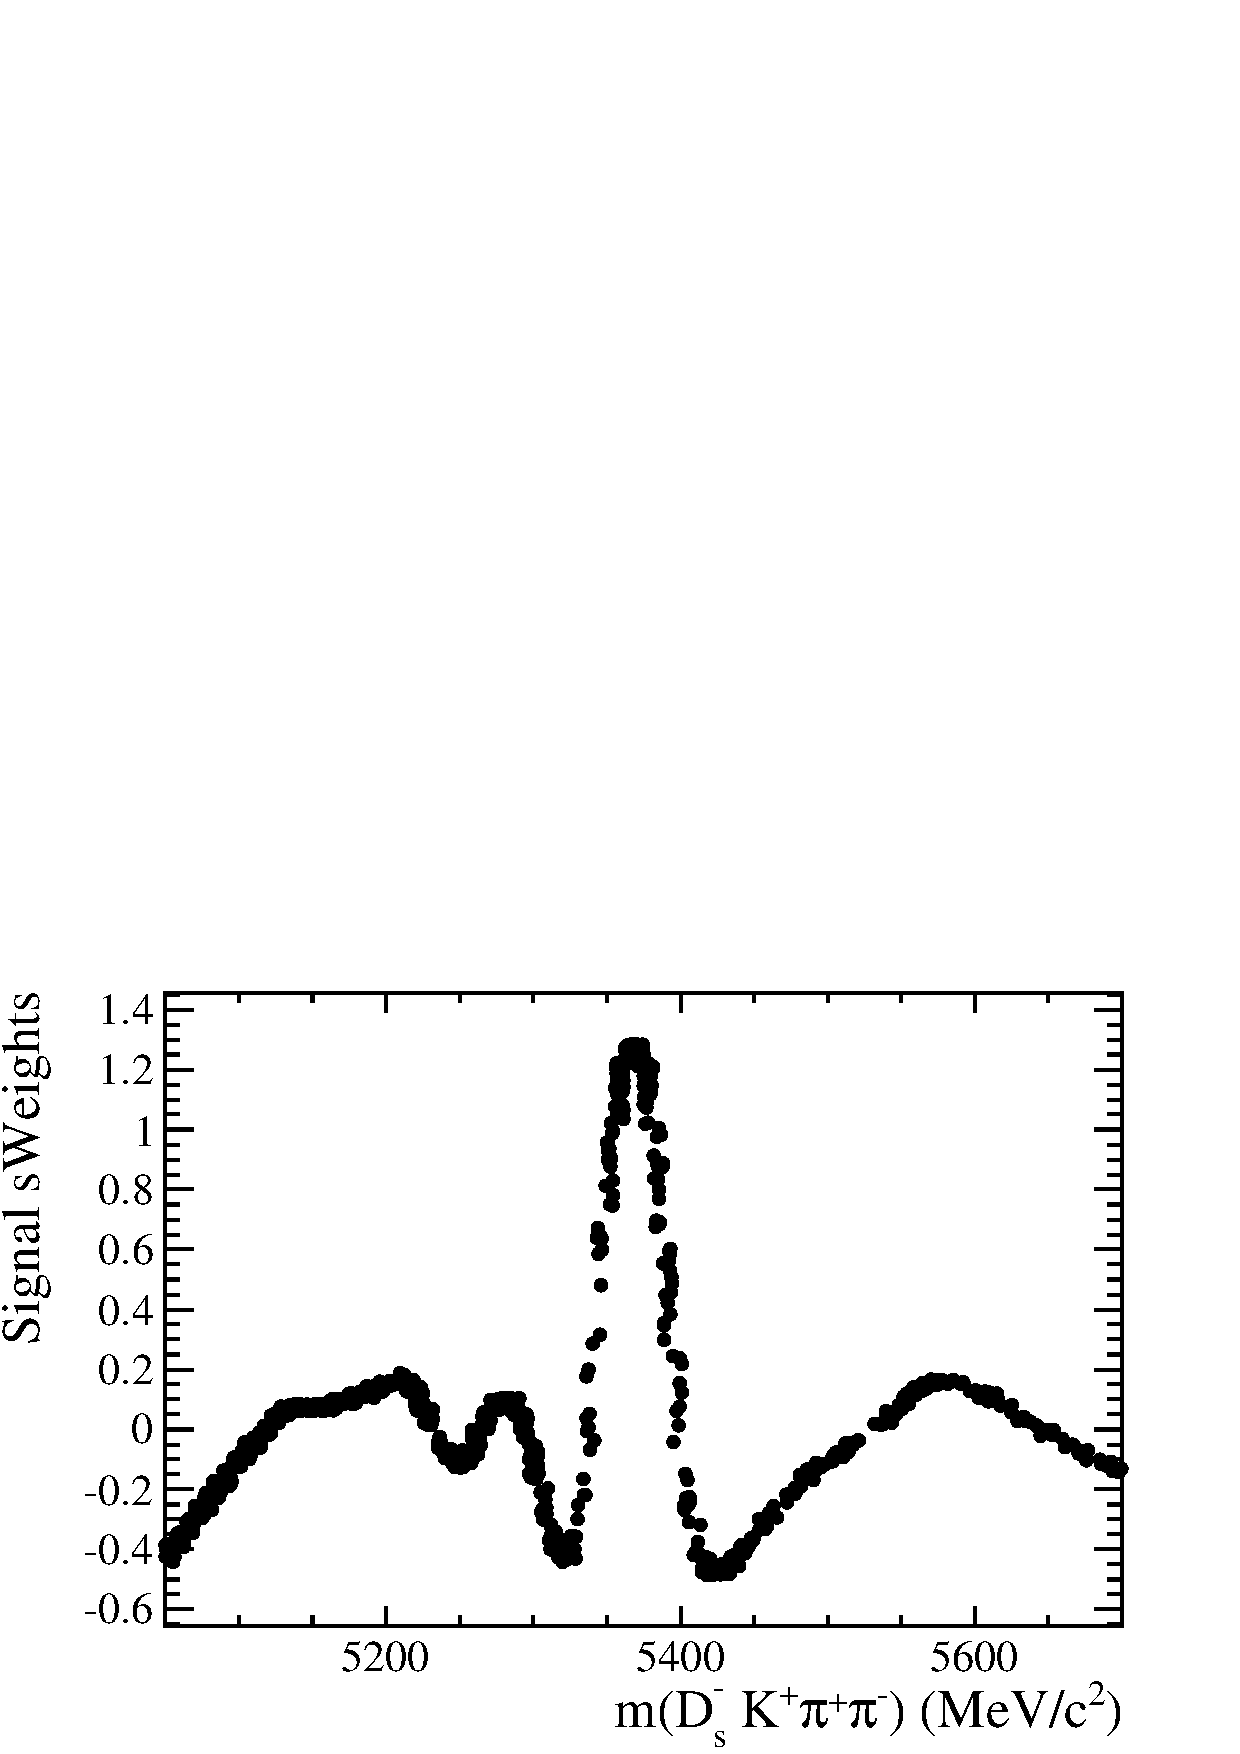
\includegraphics[height=7.cm,width=0.49\textwidth]{figs/signal_sweight_y11_phipi.pdf}
%\caption{Distribution of sWeights across the invariant mass of (left) $\Bs\to\Ds\pion\pion\pion$ and (right) $\Bs\to\Ds\kaon\pion\pion$ candidates for Run1 and Run2 data.}
%\label{fig: sWeights}
%\end{figure}
